\documentclass[math,code]{amznotes}
\setcounter{tocdepth}{1}  % Only show sections in the ToC
\usepackage[utf8]{inputenc}
\usepackage{amsmath}
\usepackage{amsfonts}
\usepackage{graphicx}
\usepackage{tikz}
\usepackage{etoolbox}
\usepackage{tabularx}
\usepackage{float} % Needed for [H] placement specifier
\usepackage{wrapfig} % Needed for wrapping figures
\usepackage{diagbox} % For diagonal split in table
\usepackage{booktabs} % For better table formatting

\graphicspath{ {./images/} }
\geometry{
    a4paper,
    headheight = 1.5cm
}

\patchcmd{\chapter}{\thispagestyle{plain}}{\thispagestyle{fancy}}{}{}

\theoremstyle{remark}
\newtheorem*{claim}{Claim}
\newtheorem*{remark}{Remark}
\newtheorem{case}{Case}

\begin{document}
\fancyhead[L]{
    Fundamentals of Project Management
}
\fancyhead[R]{
    Lecture Notes
}
\tableofcontents

\chapter{Introduction to Project Management}
\section{Introduction}
\subsection{What is project management}
\textbf{Project management} is about the \textit{project manager} applying the knowledge, skills, tools and techniques to meet the requirements of the \textit{project client.}

To do this job (project management) well, it is crucial to be familiar with the \textit{project management body of knowledge} (which is pronounced as Project Management Body of Knowledge (PIMBOK)).

\subsection{Competing project demands}
There are many stakeholders\footnote{In project management, "stakeholders" are individuals, groups, or organizations that are directly or indirectly impacted by the success or failure of a project, meaning they have a vested interest in its outcome and can influence or be influenced by the project's progress; examples include customers, managers, suppliers, investors, and community members depending on the project scope.} involved with a project, with \textbf{different needs} and \textbf{expectations}. Also, in most projects, resources are limited. Therefore, the project manager needs to strike a \textbf{balance} between the \textit{budget set} and \textit{different stakeholders' demands} with respect to project scope.

\section{What are Projects?}
\subsection{Temporal nature of projects}
Project \textit{processes} are temporary in nature and end upon the delivery or creation of the project \textit{deliverable} which can last for many year.

\subsection{Uniquess of projects}
Projects are \textbf{unique}. \textit{This is because its operating environment, resources available, stakeholders involved, constraints faced and the duration taken for its completion are different}.

However, the nature of uniqueness \textbf{doesn't mean} that the lessons learned from the completion of each of old projects \textbf{cannot} be transferred to new projects so that the same mistakes can be avoided altogether.

\subsection{Progressive elaboration and development}
All projects go through a process known as \textit{progressive elaboration and development}. This process can provide the refinements that project components (and their respective activities) pass through to reach their final state as desired by the project client.

\section{Projects, Events and Operations}
\subsection{What are projects?}
A project usually has some defined milestones and goes through a project life cycle to eventually deliver the outcome. Projects are temporary endeavors to create a unique thing.

\subsection{What are events?}
An event does not have defined milestones that go through a life cycle. However, some key dates can be indicated when some critical activities are expected to be completed.

\subsection{What are operations?}
When projects are completed, they are handed over to the clients who then manage, maintain and \textbf{operate} the completed projects. Operations are day-to-day activities that go on and on.

\section{Why are Projects Created?}
\subsection{Strategic issues for projects}
Projects are often identified based on marketplace conditions and the associated supply and demand situations. The completed projects can serve to contribute to the bottom line of a business, productivity or for a charitable cause.

\subsection{How project management is defined}
Project management is defined to mean the planning, organizing and controlling of activities to successfully accomplish the project's vision and goals. Projects typically include:
\begin{enumerate}
    \item \textbf{The project manager:} the people who are responsible for ensuring that resources are in place for project tasks to be carried out. They also plan, schedule, monitor and control each of these tasks for successful and timely completion.
    \item T\textbf{he project team:} the people who aid the project manager.
\end{enumerate}

\section{Project Management Body of Knowledge (PIMBOK)}
\subsection{What the PIMBOK encompasses}
There are \textbf{nine} areas of study in the PIMBOK.
\begin{table}[h]
    \centering
    \renewcommand{\arraystretch}{1.2}
    \begin{tabular}{|m{4.5cm}|m{4.5cm}|m{4.5cm}|}  % Adjust column width as needed
        \hline
        1. Integration Management & 2. Scope management & 3. Time management \\
        \hline
        4. Cost management & 5. Quality management & 6. Human resource management \\
        \hline
        7. Communications management & 8. Risk management & 9. Procurement management \\
        \hline
    \end{tabular}
    \caption{Project Management Knowledge Areas}
    \label{tab:chapter1-pm-knowledge-areas}
\end{table}

These nine knowledge areas are underpinned by five project management processes, which means that all these 9 areas in PIMBOK will go through the five processes below

\begin{table}[h]
    \centering
    \renewcommand{\arraystretch}{1.2}
    \begin{tabular}{|m{4.5cm}|m{4.5cm}|m{4.5cm}|}
        \hline
        1. Initiating & 2. Planning & 3. Executing \\
        \hline
        4. Monitoring and Controlling & 5. Closing & \\ 
        \hline
    \end{tabular}
    \caption{Project Management Process Groups}
    \label{tab:chapter1-pm-process-groups}
\end{table}

\subsection{Integration management}
Integration management means when a change happens, the project manager needs to understand how this change may affect all the other knowledge areas, and what therefore needs to be coordinated and integrated.

\subsection{Scope management}
This means what should be included and excluded in the project. An important outcome is the creation of a work breakdown structure to define what must be done.

\subsection{Time management}
This requires the project manager to:
\begin{enumerate}
    \item identify the tasks for the project
    \item the time taken for these tasks to be completed
    \item the sequencing of these tasks in a logical and productive manner
\end{enumerate}
The end result of time management is the creation of a project schedule with a time-line and milestones that must be controlled to meet the deadline set for project completion.

\subsection{Cost management}
Cost management includes planning, estimating, budgeting and controlling the costs of the resources used.

The outcome of cost management should be a budget or a clear picture of how much these resources cost and when the expenditure is likely to take place to avoid negative cash flow.

\subsection{Quality management}
Quality management defines and deals with how good the \textbf{service} or \textbf{product quality} should be.

\subsection{Human resource management}
Human resource management identifies the manpower needed for the project, assessing who is best positioned to take on different roles, getting them on board the project, motivating them to deliver and evaluating their performance.

To do so, organizational planning, establishing the organization structure and project team development are important issues for consideration in deciding who will do the work.

\subsection{Communications management}
Communications management is about identifying, creating and disseminating the information needed by the stakeholders at the appropriate time. And this is done via face-to-face meetings, email messages, etc.

\subsection{Risk management}
Risk management identifies, measures, analyses and recommends appropriate mitigation steps to be taken in responding to project risks.

It is necessary to strike a balance between the \textbf{impact} and the \textbf{probability} of a risk occurrence.

\subsection{Procurement management}
Procurement management establishes what need to be procured for the project and from whom. This is because projects need resources for their completion and these resources need to be procured.

For example, the project manager needs to decide:
\begin{enumerate}
    \item if such resources are to be procured from outside the organization or made within the organization.
    \item if such resources should be procured at the project level or centralized at the head office to benefit from better supplier discounts for bulk purchase.
\end{enumerate}

\section{Project Management Processes}
These five processes are usually carried out sequentially.

\subsection{Initiating}
\begin{enumerate}
    \item At the project level, initiating means activating, triggering and doing whatever is needed for the project to commence with proper authority.
    \item At the activity level, for example in procurement management, the project manager must identify what needs to be procured for the project, and then initiate actions necessary to set this process in motion.
\end{enumerate}
Initiating sets the platform for planning to take place.

\subsection{Planning}
Planning identifies all the activities and work that are required in a project for successful completion.

\subsection{Execution}
Execution means carrying out the activity or putting labor and materials together to create the work needed for the project. The completion of execution leads to the completion of one milestone for the project.

\subsection{Monitoring and controlling}
Monitoring keeps track of progress and controlling helps to keep the project on track. Monitoring and controlling are necessary to ensure that all parts of projects fall in place to meet time, cost, safety and quality targets.

\subsection{Closing}
Closing means that when an activity or work is completed, it needs to be accepted formally and the relevant stakeholders notified of the acceptance for the project to move on to another stage.

Because many different activities and works can take place at any one time in a project, the closing process is also triggered throughout the entire project duration.

\section{Beyond Project Management}
\subsection{Program management}
A program is made up of several different projects or phases contributing to a common cause.

\subsection{Portfolio management}
A portfolio is a collection of projects of a \textbf{similar} nature.

\subsection{Project Management Office (PMO)}
The project management office serves to manage, organize and control all projects undertaken by the organization.

\section{Classic Question}
\begin{enumerate}
    \item Operations can commence only with the completion of the entire project. (\textbf{FALSE})
    \item Portfolio managers do the same thing over and over again but for different projects. (\textbf{TRUE})
    \item An accidental project manager is anyone who executes projects when s/he has already completed formal training in project management. (\textbf{FALSE})
\end{enumerate}

\chapter{Project Life Cycles, Stakeholders and Organizations}
\section{Introduction}
Project life cycles are not like nature life cycle, which cannot be fast tracked. Project life cycles can be fast tracked.

\subsection{Project phasing}
Large and complex projects should be divided into phases to render the tasks more manageable. To fast track the large projects, we can overlap the phases.

\subsection{Project life cycle}
Project life cycles can vary depending on the nature of the projects. The life cycle is affected by the characteristics of the projects.

\section{Project Feasibility}
\subsection{What project feasibility studies entail}
A project starts with the identification of a perceived need or market demand. A feasibility study is then carried out to assess if the need or demand can be met realistically through the project.

\subsection{Outcomes of feasibility studies}
The outcomes can range from a simple yes or no outcome to back to the drawing board recommendations.

\section{Project Life Cycles and Phases}
\subsection{Operations of the project life cycle}
The project life cycle is typically made up of phases. The benefits of subdividing projects into phases are:
\begin{enumerate}
    \item allows the project manager to identify the nature and extent of work needed for the completion of each of these phases. This allows for the deliveries of correct materials, equipment, labor, and other resources to be made to each phase.
    \item allows the nine areas of the PIMBOK to be initiated at a manageable level for planning, executing, monitoring, controlling and closing.
    \item allows the project manager to determine which parts of the project have the most risks and must therefore be given the appropriate dose of attention.
\end{enumerate}

\subsection{Consideration for project phases}
Where time is of the essence, phases may overlap to enable fast track completion for the project.

Projects are more likely to fail at the beginning and less likely to fail towards the end of the project life cycle.

\subsection{Exiting one phase to another phase through stage gates}
Exiting a phase will require the project team to pass through an imaginary doorway commonly known as the stage gate. \textbf{Mentally}, the stage gate is where the project team exits from one phase to another phase of the project.

To pass through the stage gate of a phase, a precondition is meeting the predetermined metrics.

\section{People like You and Me}
\subsection{People as stakeholders}
Stakeholders are fundamentally people who have vested interests in the project and may act singularly as an individual or collectively as a group. They may be internal or external parties to a project.

It is crucial for project manager to identify and recognize who the various stakeholders are to understand their needs and concerns as early as possible at the project inspection stage.

\subsection{What can stakeholders do?}
Stakeholders can drive a project and also hinder the progress of a project.

\section{Organization Structures}
\subsection{How are projects organized}
Projects can be organized in many ways. There is no best way to organize a project. However, in all cases, projects are parts of larger entities set up to provide a unique product or a unique service.

There are three levels or organization emanating from the larger entities to their projects:
\begin{enumerate}
    \item \textbf{Executive level}: where the vision, mission, policies and strategies are established to achieve the wider goal of the project.
    \item \textbf{Functional level}: where a clear understanding of the project purposes is set out, and operational tactics are conceived and put in place.
    \item \textbf{Operation level}: where the operations may include decisions on how the project is going to be run.
\end{enumerate}

\subsection{Three different organization structures}
\begin{enumerate}
    \item \textbf{Functional Organization}: \\
    \begin{figure}[h]
        \centering
        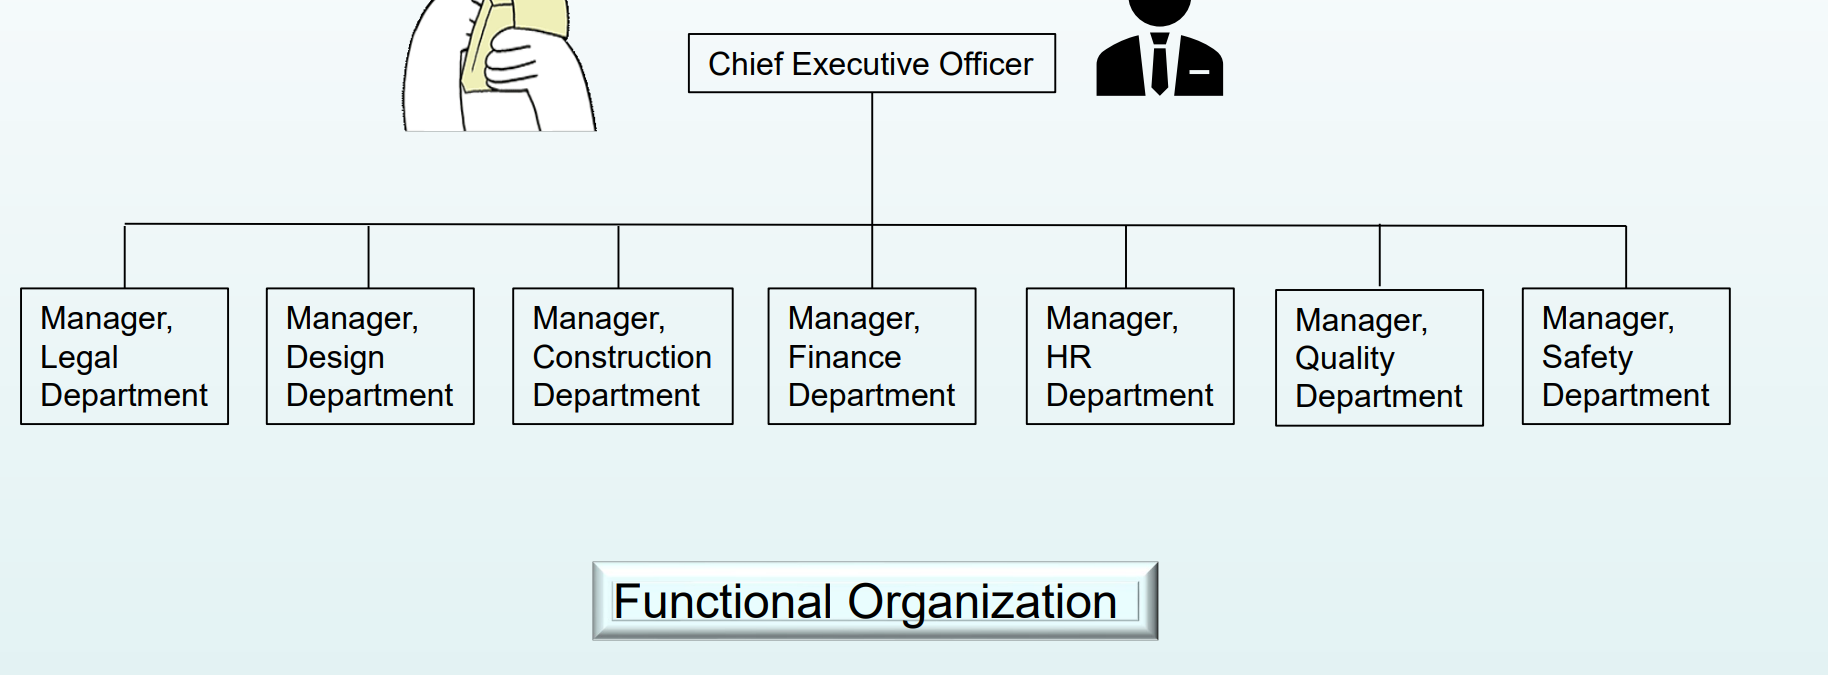
\includegraphics[width=0.75\linewidth]{images/chapter2-functional-organization.png}
        \caption{Functional Organization}
        \label{fig:chapter2-functional-organization}
    \end{figure}
    \item \textbf{Project Organization} \\
    \begin{figure}[h]
        \centering
        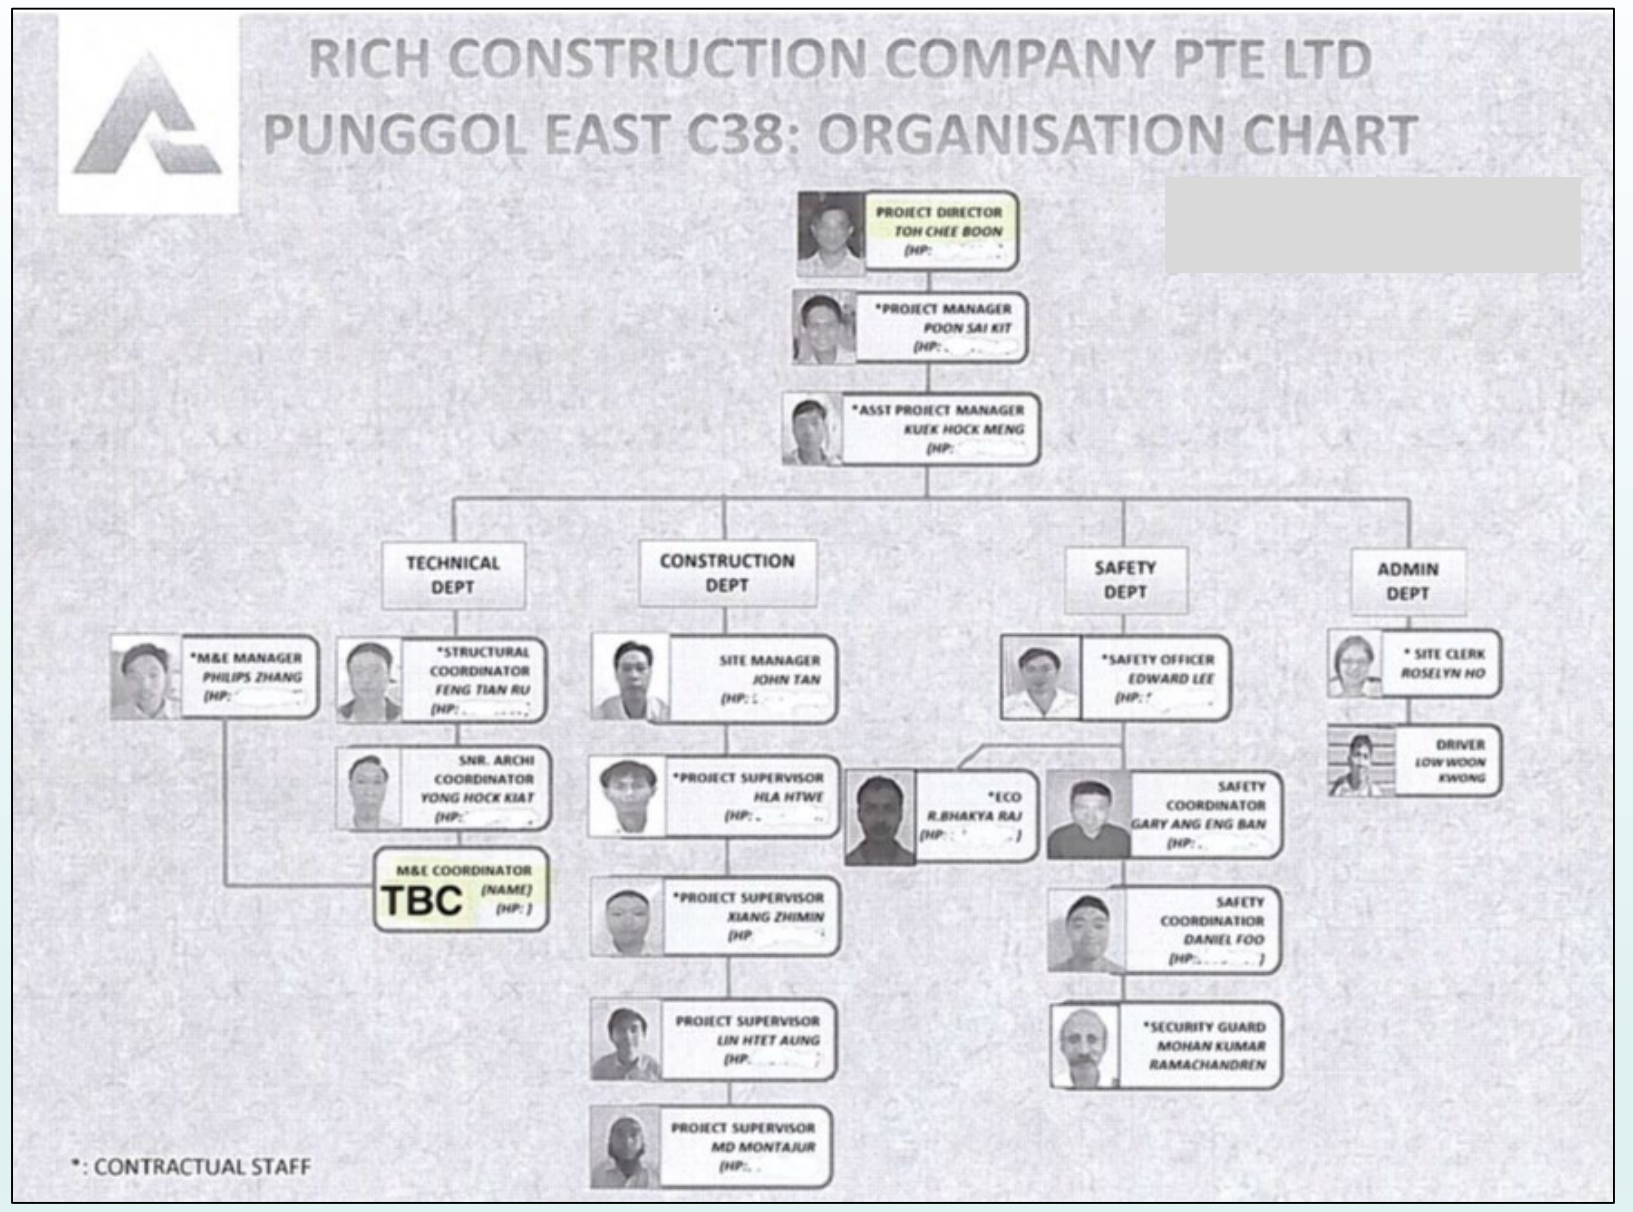
\includegraphics[width=0.75\linewidth]{chapter2-project-organization.png}
        \caption{Project Organization}
        \label{fig:chapter2-project-organization}
    \end{figure}
    \item \textbf{Matrix Structure} \\
    \begin{figure}[h]
        \centering
        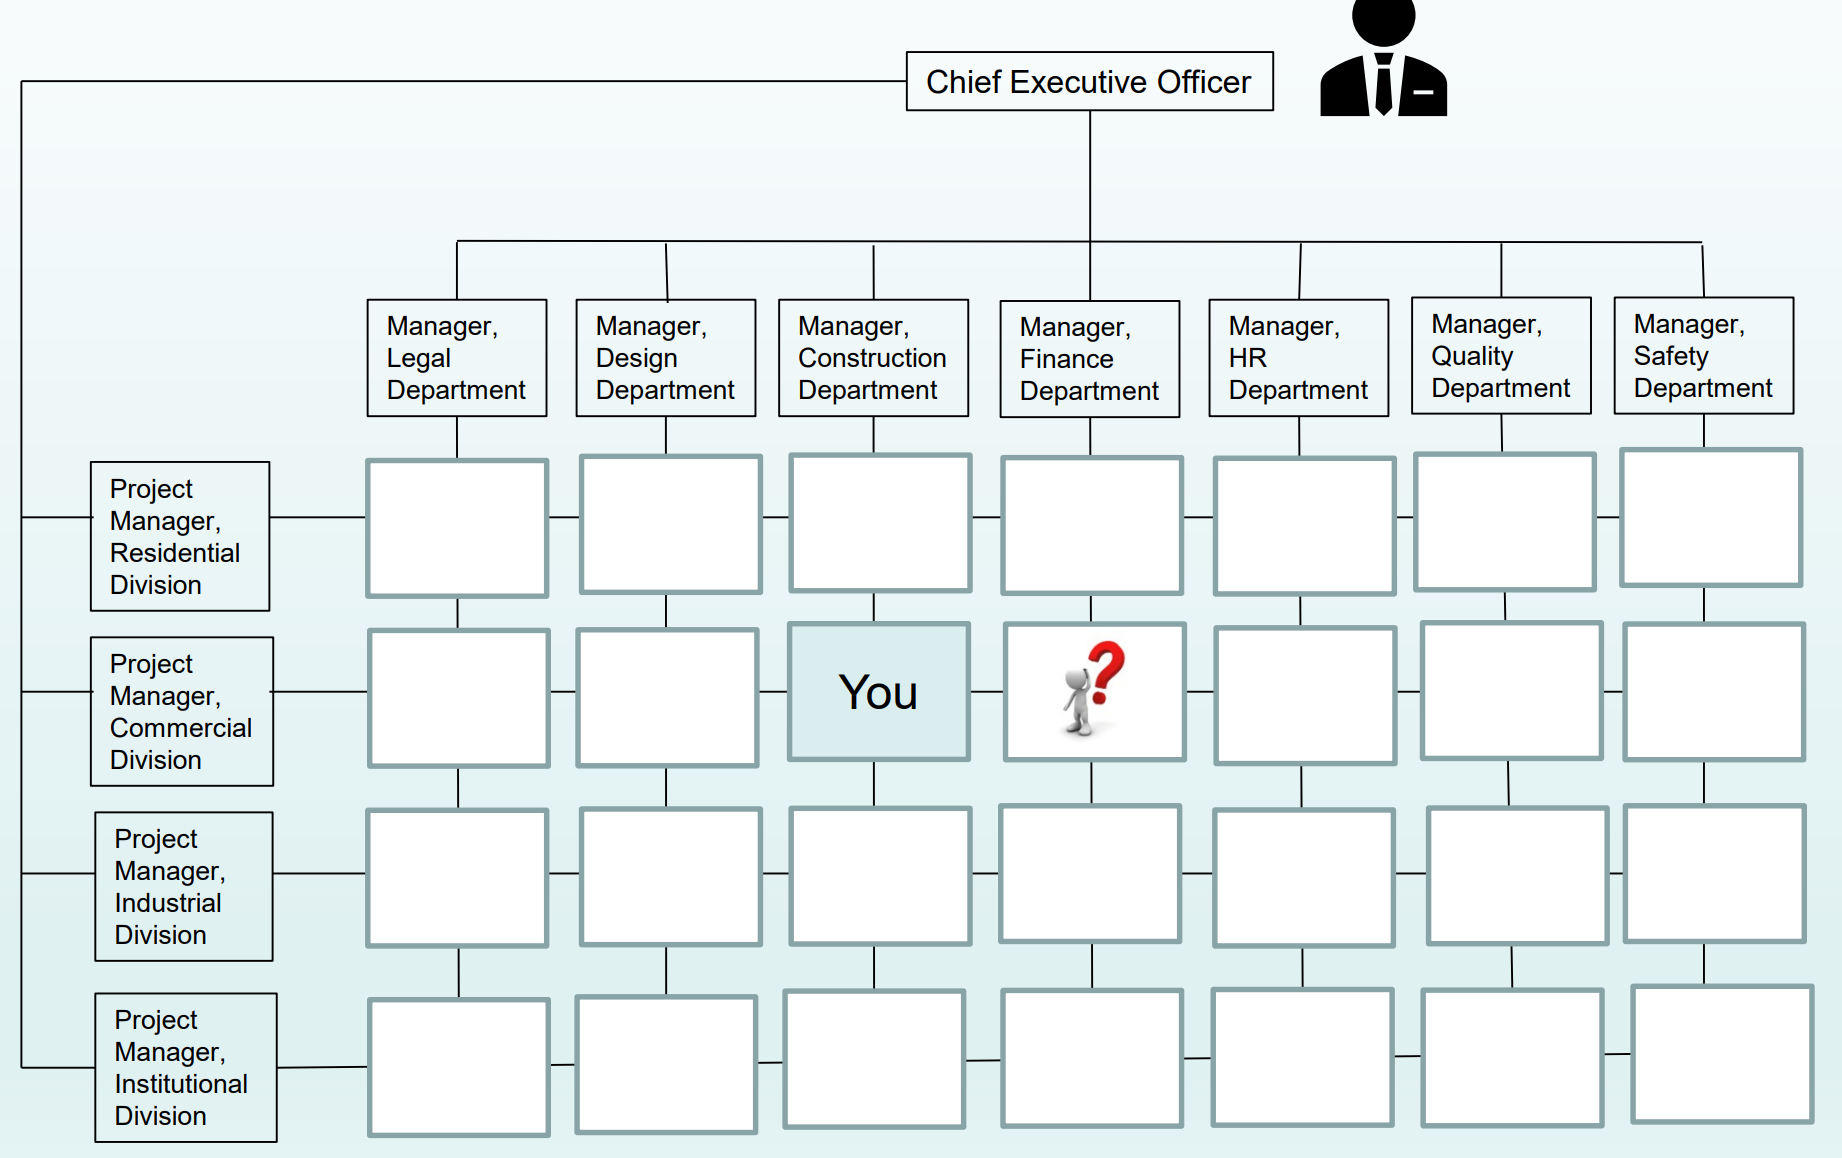
\includegraphics[width=0.75\linewidth]{images/chapter2-matrix-structure.png}
        \caption{Matrix Structure}
        \label{fig:chapter2-matrix-structure}
    \end{figure}
\end{enumerate}

\subsection{How organization structures influence authority of the project manager}
In a functional structure, project managers report directly to the functional manager to avoid confusion.

\subsection{How organization structures communicate}
A Functional structure will route information flows through the functional managers. A Project structure will route information flows through the project manager.

\subsection{Hybrid Structures}
Projects are generally organized using the functional, project or matrix structures. \textit{Hybrid structures}, are basically combinations of different structures.
\begin{figure}[h]
    \centering
    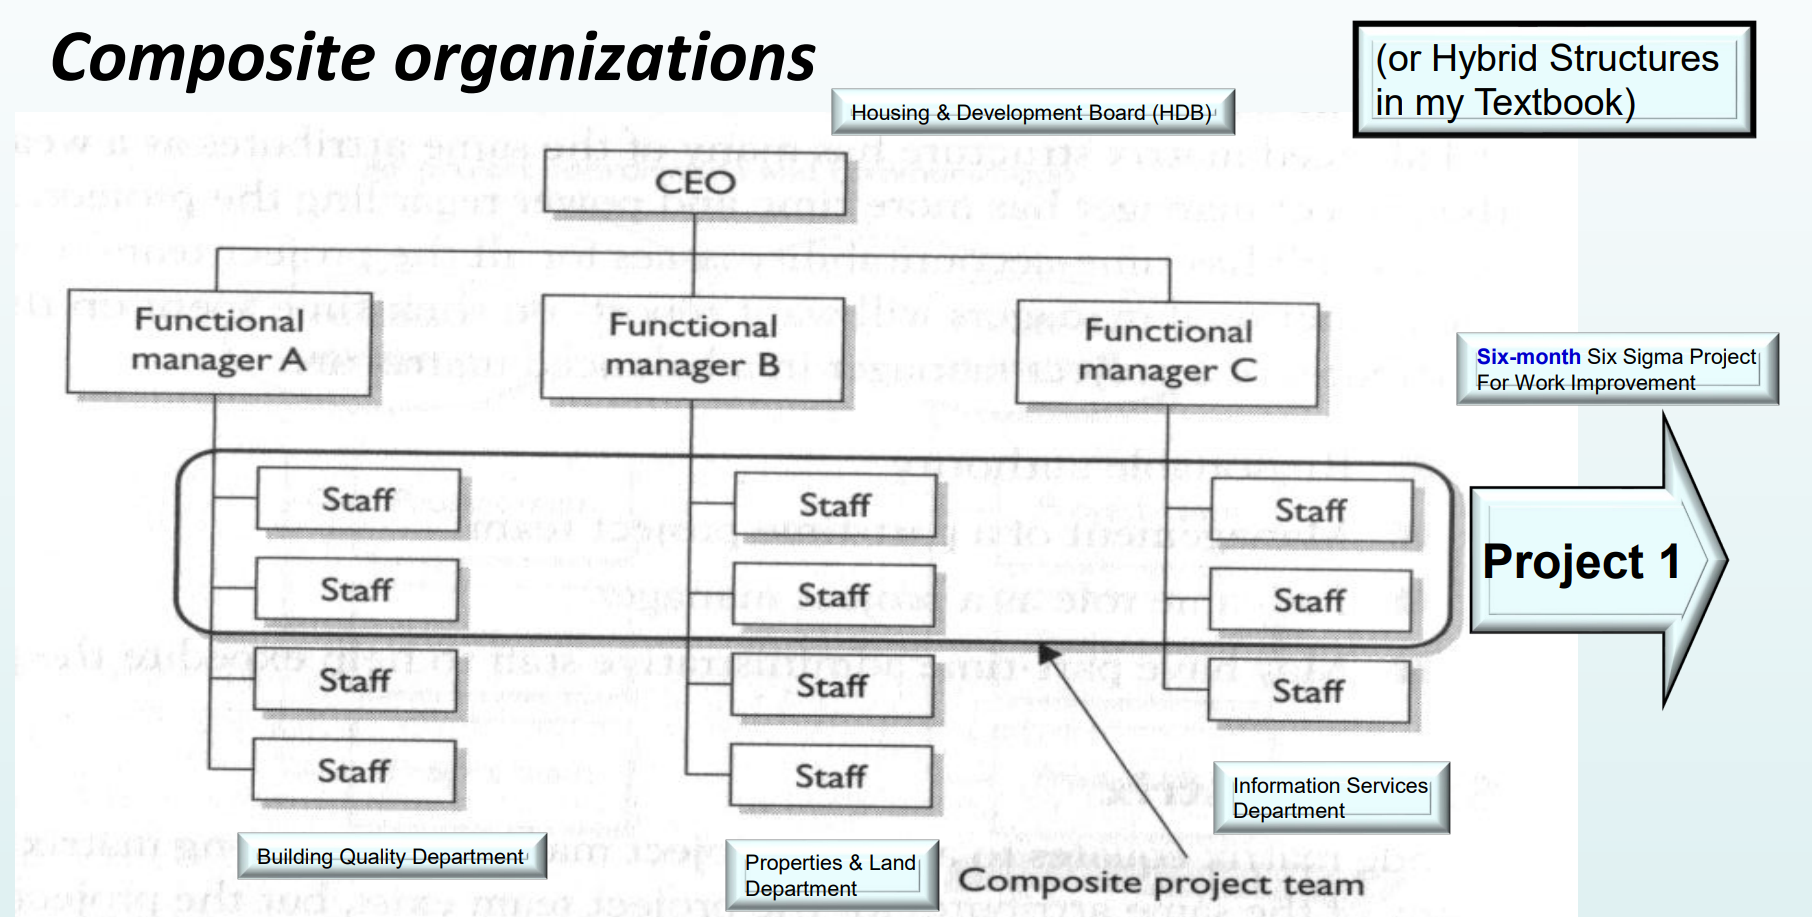
\includegraphics[width=0.75\linewidth]{images/chapter2-hybrid-structure.png}
    \caption{Hybrid Structure}
    \label{fig:chapter2-hybrid-structure}
\end{figure}

\chapter{Project Integration Management}
\section{Project Charter}
\subsection{What is Project Charter}
The project charter is an agreement that provides the \textbf{guiding principles} for the project team to \textbf{move towards the common mission}. It shows who the \textbf{major stakeholders} are and their authority to act on behalf of their respective organizations.

Once the \textbf{major issues} have been agreed, the project charter is then drafted in the form of an agreement that \textbf{sets out the key performance indicators (KPI)}\footnote{The KPI can relate to time, cost, quality targets and environment goals.} expected of the project outcome.
\subsection{What the project charter conveys}
The \textbf{project charter} serves as a communication platform for all \textbf{major stakeholders} to arrive at a common understanding of how the project is to be executed as well as the desired project outcomes. It should have:
\begin{enumerate}
    \item The KPIs we have mentioned above. All these KPIs must be fulfilled at project completion.
    \item The larger picture of the project. e.g., rebuilding or upgrading of an existing building.
    \item The key milestones so that all stakeholders are clear about the project schedule with a target time for completion.
    \item Who the various internal and external stakeholders are who may influence the project outcomes.
    \item Operating constraints.
    \item The people who are directly involved with and responsible for the successful execution of the project from inception to handover. These people may come from different functional organizations such as the HR department, accounts department, etc.
\end{enumerate}

\chapter{Project Cost Management}
\section{Introduction}
\subsection{Estimating costs of the project}
Cost estimating is the process of calculating and computing the costs of all the resources that have been identified to be necessary to complete the project. Such resources can be identified from the project scope statement, work breakdown structure, components and list of activities. Cost of these resources can be summarized into 6 M's,
\begin{enumerate}
    \item Materials
    \item Manpower
    \item Machine
    \item Management competence
    \item Methods of construction
    \item Money to fund the project
\end{enumerate}

\section{Approaches to Estimating}
\subsection{Analogous estimating}
This is also known as \textbf{top-down} approach, basically it is based on historical information of past completed projects that are quite similar to the current project.
\subsubsection{Advantages}
\begin{enumerate}
    \item It can derive quick estimates or ball-park figures requested by the client.
    \item It is useful when the project is at the early stage.
\end{enumerate}
\subsubsection{Disadvantages}
It is the least-accurate approach because of its lack of attention to details.

\subsection{Bottom-up estimating}
This is a detailed approach where each and every componenets of a project are accounted for in building up the project sum. It starts with the Work Breakdown Structure and works through all its components and activities to produce the cost estimates.
\subsubsection{Advantages}
It is time consuming.
\subsubsection{Disadvantages}
It is the most accurate.

\subsection{How costs of resources are determined}
As a Project Manager, you should go through the following \textbf{planning process} to determine the costs of resources
\begin{enumerate}
    \item \textbf{Understand what the project includes}: This is done by looking at the Work Breakdown strcture or the list of activities.
    \item \textbf{For each activity, identify the 6 M's}: namely management, method, money, materials, manpower and machinery.
    \item \textbf{Determine the quantities of these resources required}: e.g., when these are needed and should these be purchased from vendors or be made in-house.
\end{enumerate}
\begin{notebox}
    \begin{remark}
        Consider the \textbf{learning curve} when determining the costs. This means for projects with repetitive activities, workers can become more productive as they learn to do the same thing over and over again. As a result, costs may decrease as more of the same units are being built.
    \end{remark}
\end{notebox}

\chapter{Project Procurement Management}
\section{Nature of Procurement}
\subsection{What, why, how and when to procure}
Projects require a variety of resources for their completion. These resources however do not simply appear out of nowhere. They have to be procured or purchased. The project manager needs to identify and plan for what resources are necessary for the project.

\subsection{Procurement Planning}
\begin{enumerate}
    \item Some resources can be purchased from more than one supplier to avoid out-of-stock situations.
\end{enumerate}

\section{Identifying Resources for Procurement}
This starts with the \textbf{scope statement}. It can be a set of hefty documents setting out in details what is needed and therefore need to be purchased for the project.

\section{Contractual Issues}
\textbf{Procurement Contracts} should entail the following:
\begin{enumerate}
    \item All requirements set out in the contract must be fulfilled.
    \item Contracts must set out clearly what are breaches, intellectual property rights and issues relating to copyrights.
    \item Contracts should also provide for unforeseeable events that cannot be reasonably anticipated by parties such as those caused by exceptionally inclement weather and natural disasters.
\end{enumerate}

\section{Types of Contracts}
\begin{enumerate}
    \item \textbf{Fixed price contracts}: It is a procurement agreement commonly used in construction where the buyer pays the seller a predetermined lump sum for goods or services, transferring the risk of cost overruns to the seller, who must ensure accurate cost estimates and risk mitigation while the buyer bears less risk.
    \item \textbf{Cost reimbursable contracts}
    \begin{itemize}
        \item \textbf{Fixed Price Contract}: A contract type where the buyer and seller agree on a fixed total price for the project. The seller’s compensation remains unchanged regardless of actual cost variations.
        \item \textbf{Cost Reimbursable Contracts}: Contracts that allow adjustments to payments based on the seller’s actual incurred costs. The buyer reimburses the seller’s costs plus an additional fee or profit, depending on the contract type.
        \begin{itemize}
            \item \textbf{Cost Plus Fixed Fee Contract}: A contract where the seller is reimbursed for actual costs incurred, plus a predetermined fixed fee as profit. This fixed fee does not increase with project duration, incentivizing the seller to complete the work efficiently.
            \item \textbf{Cost Plus Percentage of Costs Contract}: A contract where the seller is reimbursed for actual costs and receives an additional fee calculated as a percentage of those costs. Higher costs lead to higher profits, increasing the buyer’s risk.
            \item \textbf{Cost Plus Incentive Fee Contract}: A contract where the seller is reimbursed for actual costs and earns an incentive fee based on meeting predefined targets (e.g., timely completion or cost control). This balances risk and efficiency.
        \end{itemize}
    \end{itemize}
    \item \textbf{Costs}: As we have seen from above, in cost reimbursable contract, \textbf{cost} is very important. And below summarizes the different types of costs
    \begin{itemize}
        \item \textbf{Direct Costs}: Expenses directly attributable to the project, such as salaries, equipment, and materials.
        
        \item \textbf{Indirect Costs}: Costs that support the project but are not directly tied to specific tasks, such as office rent, utilities, and overhead.
        
        \item \textbf{Profit Component}: The difference between the actual costs of goods or services and the sale price, representing the seller’s earnings. In cost reimbursable contracts, profit is paid as a fixed fee, percentage of costs, or incentive fee.
        
        \item \textbf{Cost Overruns}: Situations where actual project costs exceed the expected or budgeted amount. In cost reimbursable contracts, the buyer typically bears this risk, though the extent depends on the contract type.
    \end{itemize}
\end{enumerate}

\chapter{Group Project}
\section{Inspiration from Airplane}
\subsection{How Each Airplane Flies Autonomously}
Autonomous flight is achieved through the integrated operation of three core systems in the Automatic Flight Control System (AFCS): the Autopilot, Flight Director, and Flight Management System (FMS). These systems collaborate to handle strategic planning, tactical guidance, and precise control, enabling an aircraft to fly with minimal human intervention. Below, each system’s role and their collective workflow are detailed.

\subsubsection{Autopilot}
The autopilot automates control of the aircraft’s flight surfaces, ensuring stability and accurate maneuvering. It works with the Flight Director and FMS to follow the intended flight path.

\begin{enumerate}
    \item \textbf{First Generation Autopilot (1912)}\footnote{https://sheppardair.com/download/faa-h-8083-15B.pdf}
    \begin{itemize}
        \item \textbf{Overview:}
        \begin{itemize}
            \item Invented by Sperry in 1912.
            \item Connected gyroscopic indicators to hydraulic elevators and rudder.
            \item Kept flight straight and level automatically.
        \end{itemize}
        \item \textbf{Advantages:}
        \begin{itemize}
            \item Eased pilot workload and fatigue.
            \item Enhanced safety on long flights.
        \end{itemize}
        \item \textbf{Limitations:}
        \begin{itemize}
            \item Lacked aileron control, relying on wing dihedral for roll stability.
            \item Slow to adapt to sudden flight changes.
            \item Operated standalone, without navigation system integration.
        \end{itemize}
    \end{itemize}
    
    \item \textbf{Modern Autopilot}\footnote{https://www.boeing.com/content/dam/boeing/boeingdotcom/commercial/airports/acaps/787.pdf}
    \begin{itemize}
        \item \textbf{Integration with Other Systems:}
        \begin{itemize}
            \item Receives targets and constraints from the FMS via databus (e.g., ARINC 429).
            \item Follows Flight Director commands.
            \item Links with fly-by-wire systems in aircraft like the Airbus A350 or Boeing 787.
        \end{itemize}
        \item \textbf{Advanced Functions:}
        \begin{itemize}
            \item Performs coupled approaches using ILS/VOR data from the FMS.
            \item Coordinates thrust with FADEC systems.
            \item Manages 4D trajectories (latitude, longitude, altitude, time) with FMS input.
        \end{itemize}
        \item \textbf{Control Levels:}
        \begin{itemize}
            \item \textbf{Single-axis:} Manages roll (wing leveller).
            \item \textbf{Two-axis:} Handles roll and pitch with varying guidance levels.
            \item \textbf{Three-axis:} Adds yaw for complete flight control.
        \end{itemize}
    \end{itemize}
\end{enumerate}

\subsubsection{Flight Director}
The Flight Director (FD) provides tactical guidance, converting the FMS’s flight plan into real-time pitch and roll commands for the autopilot or pilot.

\begin{enumerate}
    \item \textbf{Main Components:}
    \begin{itemize}
        \item Command bars on the attitude indicator.
        \item Inputs from the Air Data Computer (ADC) and flight data computer.
        \item Navigation data from the FMS and other sources.
    \end{itemize}
    
    \item \textbf{How It Works:}
    \begin{itemize}
        \item Calculates pitch and bank angles needed for the flight path.
        \item Shows command cues (bars or crosshairs) for control adjustments.
        \item Directs the pilot or autopilot to align the aircraft’s attitude.
    \end{itemize}
    
    \item \textbf{Integration with Other Systems:}
    \begin{itemize}
        \item \textbf{With FMS:} Uses flight plan data to set the trajectory.
        \item \textbf{With Autopilot:} Supplies real-time signals for surface control.
        \item Supports tasks like course intercepts, altitude shifts, and crosswind handling.
    \end{itemize}
\end{enumerate}

\subsubsection{Flight Management System (FMS)}\footnote{https://www.youtube.com/watch?v=bRKyqXk9WSA}
The FMS acts as the strategic brain, automating tasks and managing the flight plan with navigation, performance, and ATC constraints.

\begin{enumerate}
    \item \textbf{Key Components:}
    \begin{itemize}
        \item Flight Management Computer (FMC).
        \item Control Display Unit (CDU).
        \item Navigation Database (waypoints, airways, procedures)\footnote{https://ffac.ch/wp-content/uploads/2020/11/ICAO-Doc-8168-Volume-I-Flight-Procedures.pdf}.
        \item Cross-talk bus linking avionics.
    \end{itemize}
    
    \item \textbf{How It Works:}
    \begin{itemize}
        \item Determines position using GPS, INS, and radio navigation.
        \item Pulls route and procedure data from the Navigation Database.
        \item Guides the aircraft along the optimal path based on real-time position and plan.
        \item Displays flight info on EFIS, Navigation Display, or Multifunction Display.
    \end{itemize}
\end{enumerate}

\subsubsection{System Integration and Workflow}
The Autopilot, Flight Director, and FMS create a closed-loop system for autonomous flight, seamlessly covering all phases from takeoff to landing.
\begin{itemize}
    \item \textbf{Strategic Level (FMS):} Builds a 4D trajectory from routes, ATC rules, and performance data.
    \item \textbf{Tactical Level (Flight Director):} Turns the trajectory into immediate control inputs.
    \item \textbf{Execution Level (Autopilot):} Acts on commands via surface controls.
\end{itemize}

\subsection{How Multiple Airplanes Fly Safely Without Colliding}
Airplanes are a vital part of global transportation, with countless aircraft crisscrossing the skies daily. To prevent collisions amidst this bustling air traffic, a combination of structured routes, expert oversight, and advanced technology ensures safety. This section explores three key mechanisms: predefined flight routes with separation standards, air traffic controllers, and the Traffic Collision Avoidance System (TCAS). The collision among the flights usually can happen in the following two parts:
\begin{enumerate}
    \item During the flight
    \item When taking off and landing
\end{enumerate}

\subsubsection{During the flying}
\begin{enumerate}
    \item \textbf{Aircraft Follow Designated Routes with Strict Separation Standards}\footnote{https://www.faa.gov/documentlibrary/media/order/atc.pdf}
    \begin{itemize}
        \item Air traffic operates much like a road network, but in three dimensions. Instead of flat, two-dimensional roads, airplanes travel along "routes"—three-dimensional corridors defined by length, width, and height. Each route has specific altitude limits, and aircraft must adhere to these boundaries while maintaining safe distances in all directions: vertically, longitudinally, and laterally.
        \item Vertically, routes are divided into altitude layers, each assigned a single direction of travel, similar to one-way streets on the ground. This prevents head-on conflicts by ensuring aircraft at the same altitude move in unison. Horizontally, aircraft maintain a minimum separation of 20 kilometers (approximately 12 miles) front-to-back, translating to a time gap of at least 10 minutes between planes. These strict standards create a robust buffer, minimizing the risk of midair collisions.
    \end{itemize}
    \item \textbf{Guidance from Air Traffic Controllers}\footnote{https://ffac.ch/wp-content/uploads/2020/10/ICAO-Annex-11-Air-Traffic-Services.pdf}: When aircraft converge at shared points along different routes—akin to vehicles at a road intersection—coordination becomes critical. Unlike roads with traffic lights, the sky relies on air traffic controllers, often called the "traffic police" of aviation. These professionals monitor radar screens, issue precise instructions, and manage aircraft movements to maintain order and prevent collisions, especially at busy junctions or airports. Their expertise ensures smooth, safe passage through crowded airspace.
    \item \textbf{TCAS: Onboard Collision Protection}\footnote{https://www.eurocontrol.int/sites/default/files/2022-03/eurocontrol-safety-acas-guide-4-1.pdf}: Beyond external oversight, aircraft are equipped with the Traffic Collision Avoidance System (TCAS), an onboard safety net. TCAS continuously scans the surrounding airspace, detecting nearby aircraft and calculating potential collision risks. If another plane approaches too closely or too quickly, TCAS alerts the pilot with visual and audible warnings, such as "Climb! Climb! Climb!" or "Descend! Descend! Descend!" If the other aircraft also has TCAS, the systems coordinate opposing maneuvers—one climbs, the other descends—ensuring a swift, effective resolution. Pilots trained to follow these prompts can confidently avoid danger, adding an extra layer of protection.
\end{enumerate}

\subsubsection{When taking off and landing}
ASF data indicate that 45 percent of collisions occur in the traffic pattern, and of these, two-thirds occur during approach and landing when aircraft are on final or over the runway\footnote{https://www.aopa.org/training-and-safety/students/presolo/skills/avoiding-midair-collisions}. 

Currently, we have the following solutions\footnote{https://www.airwaysmag.com/legacy-posts/how-airports-avoid-aircraft-collisions}:
\begin{itemize}
    \item \textbf{Air Traffic Control (ATC):} Directs aircraft via radio, ensuring safe separation during takeoff, landing, and taxiing while monitoring conflicts.
    \item \textbf{Pilot Responsibility:} Maintains situational awareness and adheres to ATC instructions, countering limited cockpit visibility.
    \item \textbf{Aircraft Marshaling:} Uses standardized hand signals from ground personnel to guide aircraft safely on the ground.
    \item \textbf{``Follow-Me'' Cars:} Guides aircraft with vehicles (e.g., yellow checkerboard vans) to designated spots at some airports.
    \item \textbf{Smart Systems:} Employs advanced visual aids and technologies to enhance ground safety and awareness.
\end{itemize}

\section{Maths Equations}
\begin{equation}
    \text{Estimated Budget}=\text{Resource Hourly Rate}\times \text{Hours}
\end{equation}
In the Resource Hourly Rate, we may have different roles, thus
\begin{align*}
    \text{Estimated Budget}&=\text{Resource Hourly Rate}\times \text{Hours}\\
    &=
    \begin{cases}
        140 & \text{if Project Manager} \\
        80 & \text{if Data Scientist}
    \end{cases}
    \times \text{Hours} \\
    &=140\times \text{Hours} + 80\times \text{Hours}
    \quad \text{(by distribution law)}
\end{align*}

\section{Individual Reflection}
\begin{enumerate}
    \item For each management, following the 5 processes. We focus more on planning. Focus on the plannning, for the other parts, a very brief introduction is enough.
\end{enumerate}
\end{document}